\documentclass[10pt]{article}
\usepackage[utf8]{inputenc}
\usepackage[T1]{fontenc}
\usepackage{amsmath}
\usepackage{amsfonts}
\usepackage{amssymb}
\usepackage[version=4]{mhchem}
\usepackage{stmaryrd}
\usepackage{graphicx}
\usepackage[export]{adjustbox}
\graphicspath{ {./images/} }
\usepackage{caption}

\begin{document}
\captionsetup{singlelinecheck=false}
\section{Axioms}
\begin{enumerate}
  \item "A is above $C, D$ is above $F$ and on $E$."
\end{enumerate}

$$
\phi_{1}: \operatorname{Above}(A, C) \wedge \operatorname{Above}(E, F) \wedge O n(D, E)
$$

\begin{enumerate}
  \setcounter{enumi}{1}
  \item "A is green while $C$ is not."
\end{enumerate}

$$
\phi_{2}: \operatorname{Green}(A) \wedge \neg \operatorname{Green}(C)
$$

\begin{enumerate}
  \setcounter{enumi}{2}
  \item "Everything is on something."
\end{enumerate}

$$
\phi_{3}: \forall x \exists y . O n(x, y)
$$

\begin{enumerate}
  \setcounter{enumi}{3}
  \item "Everything that is free has nothing on it."
\end{enumerate}

$$
\phi_{4}: \forall x .(\operatorname{Free}(x) \rightarrow \neg \exists y . \operatorname{On}(y, x))
$$

\begin{enumerate}
  \setcounter{enumi}{4}
  \item "Everything that is green is free."
\end{enumerate}

$$
\phi_{5}: \forall x .(\operatorname{Green}(x) \rightarrow \operatorname{Free}(x))
$$

\begin{enumerate}
  \setcounter{enumi}{5}
  \item "There is something that is red and is not free."
\end{enumerate}

$$
\phi_{6}: \exists x .(\operatorname{Red}(x) \wedge \neg \operatorname{Free}(x))
$$

\begin{enumerate}
  \setcounter{enumi}{6}
  \item "Everything that is not green and is above B, is red."
\end{enumerate}

$$
\phi_{7}: \forall x .(\neg \operatorname{Green}(x) \wedge \operatorname{Above}(x, B) \rightarrow \operatorname{Red}(x))
$$

\section{*}
\section{Exercise 3.13.}
Language Constants: $A, B, C, D, E, F$;\\
Predicates: On ${ }^{2}$, Above ${ }^{2}$, Free ${ }^{1}$, Red ${ }^{1}$, Green ${ }^{1}$.

Interpretation Let interpretation $\mathcal{I}_{1}$ be the following:

\begin{itemize}
  \item $\mathcal{I}_{1}(A)=b_{1}, \mathcal{I}_{1}(B)=b_{2}, \mathcal{I}_{1}(C)=b_{3}, \mathcal{I}_{1}(D)=b_{4}, \mathcal{I}_{1}(E)=b_{5}, \mathcal{I}_{1}(F)=$ table
  \item $\mathcal{I}_{1}(O n)=\left\{\left\langle b_{1}, b_{4}\right\rangle,\left\langle b_{4}, b_{3}\right\rangle,\left\langle b_{3}\right.\right.$, table $\rangle,\left\langle b_{5}, b_{2}\right\rangle,\left\langle b_{2}\right.$, table $\left.\rangle\right\}$
  \item $\mathcal{I}_{1}($ Above $)=\left\{\left\langle b_{1}, b_{4}\right\rangle,\left\langle b_{1}, b_{3}\right\rangle,\left\langle b_{1}\right.\right.$, table $\rangle,\left\langle b_{4}, b_{3}\right\rangle,\left\langle b_{4}\right.$, table $\rangle$,
\end{itemize}

$$
\left.\left\langle b_{3}, t a b l e\right\rangle,\left\langle b_{5}, b_{2}\right\rangle,\left\langle b_{5}, t a b l e\right\rangle,\left\langle b_{2}, t a b l e\right\rangle\right\}
$$

\begin{itemize}
  \item $\mathcal{I}_{1}($ Free $)=\left\{\left\langle b_{1}\right\rangle,\left\langle b_{5}\right\rangle\right\}, \mathcal{I}_{1}($ Green $)=\left\{\left\langle b_{4}\right\rangle\right\}, \mathcal{I}_{1}($ Red $)=\left\{\left\langle b_{1}\right\rangle,\left\langle b_{5}\right\rangle\right\}$\\
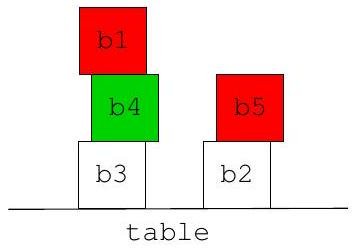
\includegraphics[max width=\textwidth, alt={}, center]{d919463b-fe47-4c21-8d15-a34b08f11db2-02_250_357_523_888}
\end{itemize}

And let interpretation $\mathcal{I}_{2}$ be:

\begin{itemize}
  \item $\mathcal{I}_{2}(A)=$ hat, $\mathcal{I}_{2}(B)=$ Joe, $\mathcal{I}_{2}(C)=$ bike, $\mathcal{I}_{2}(D)=$ Jill, $\mathcal{I}_{2}(E)=$ case, $\mathcal{I}_{2}(F)=$ ground
  \item $\mathcal{I}_{2}(O n)=\{\langle h a t$, Joe $\rangle,\langle$ Joe, bike $\rangle,\langle$ bike, ground $\rangle,\langle$ Jill, case $\rangle,\langle$ case, ground $\rangle\}$
  \item $\mathcal{I}_{2}($ Above $)=\{\langle$ hat, Joe $\rangle,\langle$ hat, bike $\rangle,\langle$ hat, ground $\rangle,\langle$ Joe, bike $\rangle,\langle$ Joe, ground $\rangle$, $\langle$ bike, ground $\rangle,\langle$ Jill, case $\rangle,\langle$ Jill, ground $\rangle,\langle$ case, ground $\rangle\}$
  \item $\mathcal{I}_{2}($ Free $)=\{\langle h a t\rangle,\langle$ Jill $\rangle\}, \mathcal{I}_{2}($ Green $)=\{\langle h a t\rangle,\langle$ ground $\rangle\}, \mathcal{I}_{2}($ Red $)=\{\langle$ bike $\rangle,\langle$ case $\rangle\}$\\
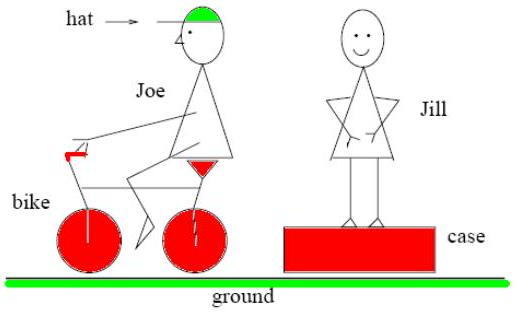
\includegraphics[max width=\textwidth, alt={}, center]{d919463b-fe47-4c21-8d15-a34b08f11db2-02_314_517_1416_813}
\end{itemize}

For each formula in Exercise 3.12, decide whether it is satisfied by $\mathcal{I}_{1}$ and /or $\mathcal{I}_{2}$.

Solution.

\begin{itemize}
  \item $\mathcal{I}_{1}=\neg \phi_{1} \wedge \neg \phi_{2} \wedge \neg \phi_{3} \wedge \phi_{4} \wedge \neg \phi_{5} \wedge \neg \phi_{6} \wedge \phi_{7}$
  \item $\mathcal{I}_{2}=\phi_{1} \wedge \phi_{2} \wedge \neg \phi_{3} \wedge \phi_{4} \wedge \neg \phi_{5} \wedge \phi_{6} \wedge \phi_{7}$
\end{itemize}

\section{Exercise 3.14.}
Consider the following sentences:

\begin{enumerate}
  \item All actors and journalists invited to the party are late.
  \item There is at least a person who is on time.
  \item There is at least an invited person who is neither a journalist nor an actor.
\end{enumerate}

Formalize the sentences and prove that 3. is not a logical consequence of 1 . and 2.

\section{Solution.}
\begin{enumerate}
  \item $\quad \forall x \cdot((a(x) \vee j(x)) \wedge i(x) \rightarrow l(x))$
  \item $\quad \exists x . \neg l(x)$
  \item $\quad \exists x .(i(x) \wedge \neg a(x) \wedge \neg j(x))$
\end{enumerate}

It's sufficient to find an interpretation $\mathcal{I}$ for which the logical consequence does not hold:

\begin{center}
\begin{tabular}{|c|c|c|c|c|}
\hline
 & $l(x)$ & $a(x)$ & $j(x)$ & $i(x)$ \\
\hline\hline
Bob & $F$ & $T$ & $F$ & $F$ \\
Tom & $T$ & $T$ & $F$ & $T$ \\
Mary & $T$ & $F$ & $T$ & $T$ \\
\hline
\end{tabular}
\end{center}

\section{*}
\section{Exercise 3.15.}
Let $\Delta=\{1,3,5,15\}$ and $\mathcal{I}$ be an interpretation on $\Delta$ interpreting the predicate symbols $E^{1}$ as 'being even', $M^{2}$ as 'being a multiple of' and $L^{2}$ as 'being less then', and s.t. $\mathcal{I}(a)=1, \mathcal{I}(b)=3, \mathcal{I}(c)=5, \mathcal{I}(d)=15$.\\
Determine whether $\mathcal{I}$ satisfies the following formulas:

\begin{enumerate}
  \item $\exists y . E(y)$
  \item $\forall x . \neg E(x)$
  \item $\forall x . M(x, a)$
  \item $\forall x . M(x, b)$
  \item $\exists x . M(x, d)$
  \item $\exists x . L(x, a)$
  \item $\forall x .(E(x) \rightarrow M(x, a))$
  \item $\forall x \exists y . L(x, y)$
  \item $\forall x \exists y . M(x, y)$
  \item $\forall x .(M(x, b) \rightarrow L(x, c))$
  \item $\forall x \forall y .(L(x, y) \rightarrow \neg L(y, x))$
  \item $\forall x .(M(x, c) \vee L(x, c))$
\end{enumerate}

Exercise 3.16.\\
Provide a First Order Logic language and a set of axioms that formalize the graph coloring problem of a graph with at most $n$ nodes, with connection degree $\leq m$, and with less then $k+1$ colors.

\begin{itemize}
  \item node degree: number of adjacent nodes
  \item connection degree of a graph: max among all the degree of its nodes
  \item graph coloring problem: given a non-oriented graph, associate a color to each of its nodes in such a way that no pair of adjacent nodes have the same color.
\end{itemize}

\section{Solution.}
\section{First Order Logic}
\section{Language}
\begin{itemize}
  \item A unary function color, where color $(x)$ is the color associated to the node x
  \item A unary predicate node, where node $(x)$ means that $x$ is a node
  \item A binary predicate edge, where edge $(x, y)$ means that $x$ is connected to $y$
\end{itemize}

\section{Axioms}
\begin{enumerate}
  \item $\forall x \forall y .(\operatorname{edge}(x, y) \rightarrow(\operatorname{color}(x) \neq \operatorname{color}(y))$\\
"Two connected node are not equally colored."
  \item $\forall x \forall x_{1} \ldots \forall x_{k+1} \cdot\left(\bigwedge_{h=1}^{k+1} \operatorname{edge}\left(x, x_{h}\right) \rightarrow \bigvee_{i, j=1, j \neq i}^{k+1} x_{i}=x_{j}\right)$\\
"A node does not have more than $k$ connected nodes."
\end{enumerate}

\section{*}
\section{Exercise 3.17.}
Let $\left\{c_{1}, . ., c_{k}\right\}$ be a non empty and finite set of colors. A partially colored directed graph is a structure $\langle N, R, C\rangle$ where

\begin{itemize}
  \item $N$ is a non empty set of nodes
  \item R is a binary relation on $N$
  \item $C$ associates colors to nodes (not all the nodes are necessarily colored,. and each node has at most one color)
\end{itemize}

Provide a first order language and a set of axioms that formalize partially colored graphs. Show that every model of this theory correspond to a partially colored graph, and vice-versa. For each of the following properties, write a formula which is true in all and only the graphs that satisfies the property:

\begin{enumerate}
  \item connected nodes don't have the same color
  \item the graph contains only 2 yellow nodes
  \item starting from a red node one can reach in at most 4 steps a green node
  \item for each color there is at least a node with this color
  \item the graph is composed of $|C|$ disjoint non empty subgraphs, one for each color
\end{enumerate}

\section{Solution.}
\section{Language}
\begin{itemize}
  \item a binary predicate edge, where edge( $n, m$ ) means that node $n$ is connected to node $m$
  \item a binary predicate color, where color $(n, x)$ means that node $n$ has color $x$
  \item the following constants: yellow, green, red
\end{itemize}

\section{Axioms}
\begin{enumerate}
  \setcounter{enumi}{-1}
  \item "each node has at most one color"
\end{enumerate}

$$
\forall n \forall x .(\operatorname{color}(n, x) \rightarrow \neg \exists y .(y \neq x \wedge \operatorname{color}(n, y)))
$$

\begin{enumerate}
  \item "connected nodes do not have the same color"
\end{enumerate}

$$
\forall n \forall m \forall x .(\operatorname{edge}(n, m) \wedge \operatorname{color}(n, x) \rightarrow \neg \operatorname{color}(m, x))
$$

\begin{enumerate}
  \setcounter{enumi}{1}
  \item "the graph contains only two yellow nodes"
\end{enumerate}

$$
\begin{array}{r}
\exists n \exists n^{\prime} .\left(\text { color }(n, \text { yellow }) \wedge \text { color }\left(n^{\prime}, \text { yellow }\right) \wedge n \neq n^{\prime} \wedge\right. \\
\left.\forall m .\left(m \neq n \wedge m \neq n^{\prime} \rightarrow \neg \operatorname{color}(m, \text { yellow })\right)\right)
\end{array}
$$

\begin{enumerate}
  \setcounter{enumi}{2}
  \item "starting from a red node one can reach in at most 4 steps a green node"
\end{enumerate}

$$
\begin{aligned}
& \forall n(\text { color }(n, \text { red }) \rightarrow \\
& \left(\exists n_{1} \cdot\left(\text { edge }\left(n, n_{1}\right) \wedge \text { color }\left(n_{1}, \text { green }\right)\right) \vee\right. \\
& \exists n_{1}, n_{2} \cdot\left(\text { edge }\left(n, n_{1}\right) \wedge \text { edge }\left(n_{1}, n_{2}\right) \wedge \text { color }\left(n_{2}, \text { green }\right)\right) \vee \\
& \exists n_{1}, n_{2}, n_{3} \cdot\left(\text { edge }\left(n, n_{1}\right) \wedge \text { edge }\left(n_{1}, n_{2}\right) \wedge \text { edge }\left(n_{2}, n_{3}\right) \wedge \operatorname{color}\left(n_{3}, \text { green }\right)\right) \vee \\
& \exists n_{1}, n_{2}, n_{3}, n_{4} \cdot\left(\text { edge }\left(n, n_{1}\right) \wedge \operatorname{edge}\left(n_{1}, n_{2}\right) \wedge \operatorname{edge}\left(n_{2}, n_{3}\right) \wedge \operatorname{edge}\left(n_{3}, n_{4}\right) \wedge \operatorname{color}\left(n_{4}, \text { green }\right)\right) \\
& ))
\end{aligned}
$$

\begin{enumerate}
  \setcounter{enumi}{3}
  \item "for each color there is at least a node with this color"
\end{enumerate}

$$
\forall x \exists n . \operatorname{color}(n, x)
$$

\begin{enumerate}
  \setcounter{enumi}{4}
  \item "the graph is composed of $|C|$ disjoint non empty subgraphs, one for each color"
\end{enumerate}

$$
\begin{aligned}
& \forall x \exists n . \operatorname{color}(n, x) \wedge \\
& \forall n \exists x . \operatorname{color}(n, x) \wedge \\
& \forall n \forall x .(\operatorname{color}(n, x) \rightarrow \neg \exists y .(y \neq x \wedge \operatorname{color}(n, y))) \wedge \\
& \forall n \forall m \forall x .(n \neq m \wedge \operatorname{color}(n, x) \wedge \operatorname{color}(m, x) \rightarrow \\
& \left.\left(\operatorname{edge}(n, m) \bigvee_{i=1}^{|N|}\left(\exists n_{1}, . ., n_{i} .\left(\operatorname{edge}\left(n, n_{1}\right) \bigwedge_{j=1}^{i-1} \operatorname{edge}\left(x_{j}, x_{j}+1\right) \wedge \operatorname{edge}\left(n_{i}, m\right)\right)\right)\right)\right)
\end{aligned}
$$

\section{*}
\section{Exercise 3.18.}
Minesweeper is a single-player computer game invented by Robert Donner in 1989. The object of the game is to clear a minefield without detonating a mine. The game screen consists of a rectangular field of squares. Each square can be cleared, or uncovered, by clicking on it. If a square that contains a mine is clicked, the game is over. If the square does not contain a mine, one of two things can happen: (1) A number between 1 and 8 appears indicating the amount of adjacent (including diagonally-adjacent) squares containing mines, or (2) no number appears; in which case there are no mines in the adjacent cells. An example of game situation is provided in the following figure:\\
Provide a first order language that allows to formalize the knowledge of a player in a game state. In such a language you should be able to formalize the following knowledge:

\begin{enumerate}
  \item there are exactly $n$ mines in the minefield
  \item if a cell contains the number 1 , then there is exactly one mine in the adjacent cells.
\end{enumerate}

\begin{figure}[h]
\begin{center}
  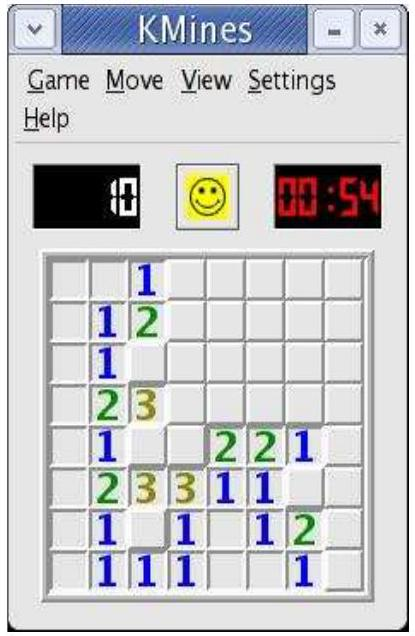
\includegraphics[alt={},max width=\textwidth]{d919463b-fe47-4c21-8d15-a34b08f11db2-08_636_415_434_858}
\captionsetup{labelformat=empty}
\caption{Figure 3.1: An example of a state in the Mines game}
\end{center}
\end{figure}

\begin{enumerate}
  \setcounter{enumi}{2}
  \item show by means of deduction that there must be a mine in the position $(3,3)$ of the game state of picture 3.1
\end{enumerate}

Suggestion: define the predicate Adj( $x, y$ ) to formalize the fact that two cells $x$ and $y$ are adjacent

\section{Solution.}
\section{Language}
\begin{enumerate}
  \item A unary predicate mine, where mine $(x)$ means that the cell xcontains a mine
  \item A binary predicate adj, where adj( $x, y$ ) means that the cell $x$ is adjacent to the cell $y$
  \item A binary predicate contains, where contains( $x, n$ ) means that the cell $x$ contains the number $n$
\end{enumerate}

\section{Axioms}
\begin{enumerate}
  \item There are exactly $n$ mines in the game.
\end{enumerate}

$$
\exists x_{1}, . . \exists x_{n}\left(\bigwedge_{i=1}^{n} \operatorname{mine}\left(x_{i}\right) \wedge \forall y\left(\operatorname{mine}(y) \rightarrow \bigvee_{i=1}^{n} y=x_{i}\right)\right)
$$

\begin{enumerate}
  \setcounter{enumi}{1}
  \item If a cell contains the number 1 , then there is exactly one mine in the adjacent cells.\\
$\forall x .(\operatorname{contains}(x, 1) \rightarrow \exists z .(\operatorname{adj}(x, z) \wedge \operatorname{mine}(z) \wedge \forall y .(\operatorname{adj}(x, y) \wedge \operatorname{mine}(y) \rightarrow y=z)))$
  \item Show by means of deduction that there must be a mine in the position $(3,3)$\\
from Picture 3.1 we have:\\
a. contains((2,2),1)\\
b. $\neg \operatorname{mine}((1,1)) \wedge \neg \operatorname{mine}((1,2)) \wedge \neg \operatorname{mine}((1,3))$\\
c. $\neg \operatorname{mine}((2,1)) \wedge \neg \operatorname{mine}((2,2)) \wedge \neg \operatorname{mine}((2,3))$\\
d. $\neg \operatorname{mine}((3,1)) \wedge \neg \operatorname{mine}((3,2))$\\
we can deduce:\\
e. $\exists z \cdot(\operatorname{adj}((2,2), z) \wedge \operatorname{mine}(z) \wedge \forall y \cdot(\operatorname{adj}((2,2), y) \wedge \operatorname{mine}(y) \rightarrow y=z)) \quad \rightsquigarrow$ from a. and axiom 2\\
f. mine $((1,1)) \vee \operatorname{mine}((1,2)) \vee \operatorname{mine}((1,3)) \vee \operatorname{mine}((2,1)) \vee \operatorname{mine}((2,2)) \vee \operatorname{mine}((2,3)) \vee \operatorname{mine}((3,1)) \vee \operatorname{mine}((3,2)) \vee \operatorname{mine}((3,3)) \rightsquigarrow$ from $e$.\\
g. mine $((3,3)) \quad \rightsquigarrow$ from b.,c.,d. and $f$.
\end{enumerate}

\begin{itemize}
  \item 
\end{itemize}

\section{Exercise 3.19.}
Formalize in first order logic the train connections in Italy. Provide a language that allows to express the fact that a town is directly connected (no intermediate train stops) with another town, by a type of train (e.g., intercity, regional, interregional). Formalize the following facts by means of axioms:

\begin{enumerate}
  \item There is no direct connection from Rome to Trento
  \item There is an intercity from Rome to Trento that stops in Firenze, Bologna and Verona.
  \item Regional trains connect towns in the same region
  \item Intercity trains don't stops in small towns.
\end{enumerate}

Solution. We define the language as follows

Constants $R M, F I, B O, V R, T N, \ldots$ are identifiers of the towns of Roma, Firenze, Bologna, Verona, Trento, . . . and InterCity, Regional, . . . are the identifiers of the type of trains

Predicates Train with arity equal to 1 , where Train $(x)$ means $x$ is a train Town with arity equal to 1 , where Train $(x)$ means $x$ is a town\\
SmallTown with arity equal to 1, where Train $(x)$ means $x$ is a small town TrainType with arity equal to 2 , where TrainType $(x, y)$ means that the train $x$ is of type $y$.\\
IsInRegion with arity equal to 2 , where IsInRegion ( $x, y$ ) means that the town $x$ is in region $y$. DirectConn with arity equal to 3, where DirectConn $(x, y, z)$ means that the train $x$ directly connects (with no intermediated stops) the towns $y$ and $z$.

Background axioms With these set of axioms we have to formalize some background knowledge which is necessary to make the formalization more adeguate

\begin{enumerate}
  \item a train has exactly one train type;
\end{enumerate}


\begin{equation*}
\forall x(\operatorname{Train}(x) \rightarrow \exists y(\operatorname{TrainType}(x, y))) \wedge \forall x y z(\operatorname{TrainType}(x, y) \wedge \operatorname{TrainType}(x, z) \rightarrow y=z) \tag{3.1}
\end{equation*}


\begin{enumerate}
  \setcounter{enumi}{1}
  \item Intercity type is different from regional type:
\end{enumerate}


\begin{equation*}
\neg(\text { InterCity }=\text { Regional }) \quad(\text { also written as InterCity } \neq \text { Regional }) \tag{3.2}
\end{equation*}


\begin{enumerate}
  \setcounter{enumi}{2}
  \item A town is associated to exactly one region
\end{enumerate}


\begin{equation*}
\forall x(\operatorname{Town}(x) \rightarrow \exists y(\operatorname{IsInRegion}(x, y))) \wedge \forall x y z(\operatorname{IsInRegion}(x, y) \wedge \operatorname{IsInRegion}(x, z) \rightarrow y=z) \tag{3.3}
\end{equation*}



\end{document}
